
%% bare_conf.tex
%% V1.3
%% 2007/01/11
%% by Michael Shell
%% See:
%% http://www.michaelshell.org/
%% for current contact information.
%%
%% This is a skeleton file demonstrating the use of IEEEtran.cls
%% (requires IEEEtran.cls version 1.7 or later) with an IEEE conference paper.
%%
%% Support sites:
%% http://www.michaelshell.org/tex/ieeetran/
%% http://www.ctan.org/tex-archive/macros/latex/contrib/IEEEtran/
%% and
%% http://www.ieee.org/

%%*************************************************************************
%% Legal Notice:
%% This code is offered as-is without any warranty either expressed or
%% implied; without even the implied warranty of MERCHANTABILITY or
%% FITNESS FOR A PARTICULAR PURPOSE!
%% User assumes all risk.
%% In no event shall IEEE or any contributor to this code be liable for
%% any damages or losses, including, but not limited to, incidental,
%% consequential, or any other damages, resulting from the use or misuse
%% of any information contained here.
%%
%% All comments are the opinions of their respective authors and are not
%% necessarily endorsed by the IEEE.
%%
%% This work is distributed under the LaTeX Project Public License (LPPL)
%% ( http://www.latex-project.org/ ) version 1.3, and may be freely used,
%% distributed and modified. A copy of the LPPL, version 1.3, is included
%% in the base LaTeX documentation of all distributions of LaTeX released
%% 2003/12/01 or later.
%% Retain all contribution notices and credits.
%% ** Modified files should be clearly indicated as such, including  **
%% ** renaming them and changing author support contact information. **
%%
%% File list of work: IEEEtran.cls, IEEEtran_HOWTO.pdf, bare_adv.tex,
%%                    bare_conf.tex, bare_jrnl.tex, bare_jrnl_compsoc.tex
%%*************************************************************************

% *** Authors should verify (and, if needed, correct) their LaTeX system  ***
% *** with the testflow diagnostic prior to trusting their LaTeX platform ***
% *** with production work. IEEE's font choices can trigger bugs that do  ***
% *** not appear when using other class files.                            ***
% The testflow support page is at:
% http://www.michaelshell.org/tex/testflow/



% Note that the a4paper option is mainly intended so that authors in
% countries using A4 can easily print to A4 and see how their papers will
% look in print - the typesetting of the document will not typically be
% affected with changes in paper size (but the bottom and side margins will).
% Use the testflow package mentioned above to verify correct handling of
% both paper sizes by the user's LaTeX system.
%
% Also note that the "draftcls" or "draftclsnofoot", not "draft", option
% should be used if it is desired that the figures are to be displayed in
% draft mode.
%
\documentclass[conference]{IEEEtran}
\usepackage{amsmath}
\usepackage{mathtools}
\usepackage{tikz}
\usepackage{pgfplots}
\usepackage{xcolor}
\usepackage{rotating}

% Add the compsoc option for Computer Society conferences.
%
% If IEEEtran.cls has not been installed into the LaTeX system files,
% manually specify the path to it like:
% \documentclass[conference]{../sty/IEEEtran}





% Some very useful LaTeX packages include:
% (uncomment the ones you want to load)


% *** MISC UTILITY PACKAGES ***
%
%\usepackage{ifpdf}
% Heiko Oberdiek's ifpdf.sty is very useful if you need conditional
% compilation based on whether the output is pdf or dvi.
% usage:
% \ifpdf
%   % pdf code
% \else
%   % dvi code
% \fi
% The latest version of ifpdf.sty can be obtained from:
% http://www.ctan.org/tex-archive/macros/latex/contrib/oberdiek/
% Also, note that IEEEtran.cls V1.7 and later provides a builtin
% \ifCLASSINFOpdf conditional that works the same way.
% When switching from latex to pdflatex and vice-versa, the compiler may
% have to be run twice to clear warning/error messages.






% *** CITATION PACKAGES ***
%
%\usepackage{cite}
% cite.sty was written by Donald Arseneau
% V1.6 and later of IEEEtran pre-defines the format of the cite.sty package
% \cite{} output to follow that of IEEE. Loading the cite package will
% result in citation numbers being automatically sorted and properly
% "compressed/ranged". e.g., [1], [9], [2], [7], [5], [6] without using
% cite.sty will become [1], [2], [5]--[7], [9] using cite.sty. cite.sty's
% \cite will automatically add leading space, if needed. Use cite.sty's
% noadjust option (cite.sty V3.8 and later) if you want to turn this off.
% cite.sty is already installed on most LaTeX systems. Be sure and use
% version 4.0 (2003-05-27) and later if using hyperref.sty. cite.sty does
% not currently provide for hyperlinked citations.
% The latest version can be obtained at:
% http://www.ctan.org/tex-archive/macros/latex/contrib/cite/
% The documentation is contained in the cite.sty file itself.






% *** GRAPHICS RELATED PACKAGES ***
%
\ifCLASSINFOpdf
  % \usepackage[pdftex]{graphicx}
  % declare the path(s) where your graphic files are
  % \graphicspath{{../pdf/}{../jpeg/}}
  % and their extensions so you won't have to specify these with
  % every instance of \includegraphics
  % \DeclareGraphicsExtensions{.pdf,.jpeg,.png}
\else
  % or other class option (dvipsone, dvipdf, if not using dvips). graphicx
  % will default to the driver specified in the system graphics.cfg if no
  % driver is specified.
  % \usepackage[dvips]{graphicx}
  % declare the path(s) where your graphic files are
  % \graphicspath{{../eps/}}
  % and their extensions so you won't have to specify these with
  % every instance of \includegraphics
  % \DeclareGraphicsExtensions{.eps}
\fi
% graphicx was written by David Carlisle and Sebastian Rahtz. It is
% required if you want graphics, photos, etc. graphicx.sty is already
% installed on most LaTeX systems. The latest version and documentation can
% be obtained at:
% http://www.ctan.org/tex-archive/macros/latex/required/graphics/
% Another good source of documentation is "Using Imported Graphics in
% LaTeX2e" by Keith Reckdahl which can be found as epslatex.ps or
% epslatex.pdf at: http://www.ctan.org/tex-archive/info/
%
% latex, and pdflatex in dvi mode, support graphics in encapsulated
% postscript (.eps) format. pdflatex in pdf mode supports graphics
% in .pdf, .jpeg, .png and .mps (metapost) formats. Users should ensure
% that all non-photo figures use a vector format (.eps, .pdf, .mps) and
% not a bitmapped formats (.jpeg, .png). IEEE frowns on bitmapped formats
% which can result in "jaggedy"/blurry rendering of lines and letters as
% well as large increases in file sizes.
%
% You can find documentation about the pdfTeX application at:
% http://www.tug.org/applications/pdftex





% *** MATH PACKAGES ***
%
%\usepackage[cmex10]{amsmath}
% A popular package from the American Mathematical Society that provides
% many useful and powerful commands for dealing with mathematics. If using
% it, be sure to load this package with the cmex10 option to ensure that
% only type 1 fonts will utilized at all point sizes. Without this option,
% it is possible that some math symbols, particularly those within
% footnotes, will be rendered in bitmap form which will result in a
% document that can not be IEEE Xplore compliant!
%
% Also, note that the amsmath package sets \interdisplaylinepenalty to 10000
% thus preventing page breaks from occurring within multiline equations. Use:
%\interdisplaylinepenalty=2500
% after loading amsmath to restore such page breaks as IEEEtran.cls normally
% does. amsmath.sty is already installed on most LaTeX systems. The latest
% version and documentation can be obtained at:
% http://www.ctan.org/tex-archive/macros/latex/required/amslatex/math/





% *** SPECIALIZED LIST PACKAGES ***
%
%\usepackage{algorithmic}
% algorithmic.sty was written by Peter Williams and Rogerio Brito.
% This package provides an algorithmic environment fo describing algorithms.
% You can use the algorithmic environment in-text or within a figure
% environment to provide for a floating algorithm. Do NOT use the algorithm
% floating environment provided by algorithm.sty (by the same authors) or
% algorithm2e.sty (by Christophe Fiorio) as IEEE does not use dedicated
% algorithm float types and packages that provide these will not provide
% correct IEEE style captions. The latest version and documentation of
% algorithmic.sty can be obtained at:
% http://www.ctan.org/tex-archive/macros/latex/contrib/algorithms/
% There is also a support site at:
% http://algorithms.berlios.de/index.html
% Also of interest may be the (relatively newer and more customizable)
% algorithmicx.sty package by Szasz Janos:
% http://www.ctan.org/tex-archive/macros/latex/contrib/algorithmicx/




% *** ALIGNMENT PACKAGES ***
%
%\usepackage{array}
% Frank Mittelbach's and David Carlisle's array.sty patches and improves
% the standard LaTeX2e array and tabular environments to provide better
% appearance and additional user controls. As the default LaTeX2e table
% generation code is lacking to the point of almost being broken with
% respect to the quality of the end results, all users are strongly
% advised to use an enhanced (at the very least that provided by array.sty)
% set of table tools. array.sty is already installed on most systems. The
% latest version and documentation can be obtained at:
% http://www.ctan.org/tex-archive/macros/latex/required/tools/


%\usepackage{mdwmath}
%\usepackage{mdwtab}
% Also highly recommended is Mark Wooding's extremely powerful MDW tools,
% especially mdwmath.sty and mdwtab.sty which are used to format equations
% and tables, respectively. The MDWtools set is already installed on most
% LaTeX systems. The lastest version and documentation is available at:
% http://www.ctan.org/tex-archive/macros/latex/contrib/mdwtools/


% IEEEtran contains the IEEEeqnarray family of commands that can be used to
% generate multiline equations as well as matrices, tables, etc., of high
% quality.


%\usepackage{eqparbox}
% Also of notable interest is Scott Pakin's eqparbox package for creating
% (automatically sized) equal width boxes - aka "natural width parboxes".
% Available at:
% http://www.ctan.org/tex-archive/macros/latex/contrib/eqparbox/





% *** SUBFIGURE PACKAGES ***
%\usepackage[tight,footnotesize]{subfigure}
% subfigure.sty was written by Steven Douglas Cochran. This package makes it
% easy to put subfigures in your figures. e.g., "Figure 1a and 1b". For IEEE
% work, it is a good idea to load it with the tight package option to reduce
% the amount of white space around the subfigures. subfigure.sty is already
% installed on most LaTeX systems. The latest version and documentation can
% be obtained at:
% http://www.ctan.org/tex-archive/obsolete/macros/latex/contrib/subfigure/
% subfigure.sty has been superceeded by subfig.sty.



%\usepackage[caption=false]{caption}
%\usepackage[font=footnotesize]{subfig}
% subfig.sty, also written by Steven Douglas Cochran, is the modern
% replacement for subfigure.sty. However, subfig.sty requires and
% automatically loads Axel Sommerfeldt's caption.sty which will override
% IEEEtran.cls handling of captions and this will result in nonIEEE style
% figure/table captions. To prevent this problem, be sure and preload
% caption.sty with its "caption=false" package option. This is will preserve
% IEEEtran.cls handing of captions. Version 1.3 (2005/06/28) and later
% (recommended due to many improvements over 1.2) of subfig.sty supports
% the caption=false option directly:
%\usepackage[caption=false,font=footnotesize]{subfig}
%
% The latest version and documentation can be obtained at:
% http://www.ctan.org/tex-archive/macros/latex/contrib/subfig/
% The latest version and documentation of caption.sty can be obtained at:
% http://www.ctan.org/tex-archive/macros/latex/contrib/caption/




% *** FLOAT PACKAGES ***
%
%\usepackage{fixltx2e}
% fixltx2e, the successor to the earlier fix2col.sty, was written by
% Frank Mittelbach and David Carlisle. This package corrects a few problems
% in the LaTeX2e kernel, the most notable of which is that in current
% LaTeX2e releases, the ordering of single and double column floats is not
% guaranteed to be preserved. Thus, an unpatched LaTeX2e can allow a
% single column figure to be placed prior to an earlier double column
% figure. The latest version and documentation can be found at:
% http://www.ctan.org/tex-archive/macros/latex/base/



%\usepackage{stfloats}
% stfloats.sty was written by Sigitas Tolusis. This package gives LaTeX2e
% the ability to do double column floats at the bottom of the page as well
% as the top. (e.g., "\begin{figure*}[!b]" is not normally possible in
% LaTeX2e). It also provides a command:
%\fnbelowfloat
% to enable the placement of footnotes below bottom floats (the standard
% LaTeX2e kernel puts them above bottom floats). This is an invasive package
% which rewrites many portions of the LaTeX2e float routines. It may not work
% with other packages that modify the LaTeX2e float routines. The latest
% version and documentation can be obtained at:
% http://www.ctan.org/tex-archive/macros/latex/contrib/sttools/
% Documentation is contained in the stfloats.sty comments as well as in the
% presfull.pdf file. Do not use the stfloats baselinefloat ability as IEEE
% does not allow \baselineskip to stretch. Authors submitting work to the
% IEEE should note that IEEE rarely uses double column equations and
% that authors should try to avoid such use. Do not be tempted to use the
% cuted.sty or midfloat.sty packages (also by Sigitas Tolusis) as IEEE does
% not format its papers in such ways.





% *** PDF, URL AND HYPERLINK PACKAGES ***
%
%\usepackage{url}
% url.sty was written by Donald Arseneau. It provides better support for
% handling and breaking URLs. url.sty is already installed on most LaTeX
% systems. The latest version can be obtained at:
% http://www.ctan.org/tex-archive/macros/latex/contrib/misc/
% Read the url.sty source comments for usage information. Basically,
% \url{my_url_here}.





% *** Do not adjust lengths that control margins, column widths, etc. ***
% *** Do not use packages that alter fonts (such as pslatex).         ***
% There should be no need to do such things with IEEEtran.cls V1.6 and later.
% (Unless specifically asked to do so by the journal or conference you plan
% to submit to, of course. )


% correct bad hyphenation here
\hyphenation{op-tical net-works semi-conduc-tor}


\begin{document}


\definecolor{fourth}{RGB}{74,105,135}
\definecolor{fifth}{RGB}{132,169,205}
\definecolor{third}{RGB}{152,95,106}
\definecolor{seventh}{RGB}{157,132,147}
\definecolor{first}{RGB}{255,206,115}
\definecolor{second}{RGB}{255,121,134}
\definecolor{sixth}{RGB}{133,173,142}
%
% paper title
% can use linebreaks \\ within to get better formatting as desired
\title{Advanced Computer Architecture \\ The ''Smooth'' Challenge}

% author names and affiliations
% use a multiple column layout for up to three different
% affiliations
\author{\IEEEauthorblockN{Lukasz Koprowski}
\IEEEauthorblockA{Department of Computing\\
Imperial College London\\
Email: lukasz.koprowski10@imperial.ac.uk}
\and
\IEEEauthorblockN{Robert Kruszewski}
\IEEEauthorblockA{Department of Computing\\
Imperial College London\\
Email: robert.kruszewski10@imperial.ac.uk}}


% conference papers do not typically use \thanks and this command
% is locked out in conference mode. If really needed, such as for
% the acknowledgment of grants, issue a \IEEEoverridecommandlockouts
% after \documentclass

% for over three affiliations, or if they all won't fit within the width
% of the page, use this alternative format:
%
%\author{\IEEEauthorblockN{Michael Shell\IEEEauthorrefmark{1},
%Homer Simpson\IEEEauthorrefmark{2},
%James Kirk\IEEEauthorrefmark{3},
%Montgomery Scott\IEEEauthorrefmark{3} and
%Eldon Tyrell\IEEEauthorrefmark{4}}
%\IEEEauthorblockA{\IEEEauthorrefmark{1}School of Electrical and Computer Engineering\\
%Georgia Institute of Technology,
%Atlanta, Georgia 30332--0250\\ Email: see http://www.michaelshell.org/contact.html}
%\IEEEauthorblockA{\IEEEauthorrefmark{2}Twentieth Century Fox, Springfield, USA\\
%Email: homer@thesimpsons.com}
%\IEEEauthorblockA{\IEEEauthorrefmark{3}Starfleet Academy, San Francisco, California 96678-2391\\
%Telephone: (800) 555--1212, Fax: (888) 555--1212}
%\IEEEauthorblockA{\IEEEauthorrefmark{4}Tyrell Inc., 123 Replicant Street, Los Angeles, California 90210--4321}}


% use for special paper notices
%\IEEEspecialpapernotice{(Invited Paper)}


% make the title area
\maketitle


\begin{abstract}
Our task was to speed up given application us much possible.
During three weeks we worked on improving its performance by utilizing as much hardware power as possible and optimizing software.
We have achieved eightfold improvement adapting sequential code for multi threaded execution and using compiler to generate the fastest possible code for our architecture.
We evaluated our progress by benchmarking the application multiple times on two sizes of the problem, after each major improvement.
\end{abstract}



% For peer review papers, you can put extra information on the cover
% page as needed:
% \ifCLASSOPTIONpeerreview
% \begin{center} \bfseries EDICS Category: 3-BBND \end{center}
% \fi
%
% For peerreview papers, this IEEEtran command inserts a page break and
% creates the second title. It will be ignored for other modes.
\IEEEpeerreviewmaketitle



% \section{Introduction}
% % no \IEEEPARstart
% This demo file is intended to serve as a ``starter file''
% for IEEE conference papers produced under \LaTeX\ using
% IEEEtran.cls version 1.7 and later.
% % You must have at least 2 lines in the paragraph with the drop letter
% % (should never be an issue)
% I wish you the best of success.

% \hfill mds

% \hfill January 11, 2007

% \subsection{Subsection Heading Here}
% Subsection text here.


% \subsubsection{Subsubsection Heading Here}
% Subsubsection text here.


% An example of a floating figure using the graphicx package.
% Note that \label must occur AFTER (or within) \caption.
% For figures, \caption should occur after the \includegraphics.
% Note that IEEEtran v1.7 and later has special internal code that
% is designed to preserve the operation of \label within \caption
% even when the captionsoff option is in effect. However, because
% of issues like this, it may be the safest practice to put all your
% \label just after \caption rather than within \caption{}.
%
% Reminder: the "draftcls" or "draftclsnofoot", not "draft", class
% option should be used if it is desired that the figures are to be
% displayed while in draft mode.
%
%\begin{figure}[!t]
%\centering
%\includegraphics[width=2.5in]{myfigure}
% where an .eps filename suffix will be assumed under latex,
% and a .pdf suffix will be assumed for pdflatex; or what has been declared
% via \DeclareGraphicsExtensions.
%\caption{Simulation Results}
%\label{fig_sim}
%\end{figure}

% Note that IEEE typically puts floats only at the top, even when this
% results in a large percentage of a column being occupied by floats.


% An example of a double column floating figure using two subfigures.
% (The subfig.sty package must be loaded for this to work.)
% The subfigure \label commands are set within each subfloat command, the
% \label for the overall figure must come after \caption.
% \hfil must be used as a separator to get equal spacing.
% The subfigure.sty package works much the same way, except \subfigure is
% used instead of \subfloat.
%
%\begin{figure*}[!t]
%\centerline{\subfloat[Case I]\includegraphics[width=2.5in]{subfigcase1}%
%\label{fig_first_case}}
%\hfil
%\subfloat[Case II]{\includegraphics[width=2.5in]{subfigcase2}%
%\label{fig_second_case}}}
%\caption{Simulation results}
%\label{fig_sim}
%\end{figure*}
%
% Note that often IEEE papers with subfigures do not employ subfigure
% captions (using the optional argument to \subfloat), but instead will
% reference/describe all of them (a), (b), etc., within the main caption.


% An example of a floating table. Note that, for IEEE style tables, the
% \caption command should come BEFORE the table. Table text will default to
% \footnotesize as IEEE normally uses this smaller font for tables.
% The \label must come after \caption as always.
%
%\begin{table}[!t]
%% increase table row spacing, adjust to taste
%\renewcommand{\arraystretch}{1.3}
% if using array.sty, it might be a good idea to tweak the value of
% \extrarowheight as needed to properly center the text within the cells
%\caption{An Example of a Table}
%\label{table_example}
%\centering
%% Some packages, such as MDW tools, offer better commands for making tables
%% than the plain LaTeX2e tabular which is used here.
%\begin{tabular}{|c||c|}
%\hline
%One & Two\\
%\hline
%Three & Four\\
%\hline
%\end{tabular}
%\end{table}


% Note that IEEE does not put floats in the very first column - or typically
% anywhere on the first page for that matter. Also, in-text middle ("here")
% positioning is not used. Most IEEE journals/conferences use top floats
% exclusively. Note that, LaTeX2e, unlike IEEE journals/conferences, places
% footnotes above bottom floats. This can be corrected via the \fnbelowfloat
% command of the stfloats package.

\section{Hardware and Software Analysis}

We have decided to use our lab machines as they are in abundance making testing easier.
Also as they are modern and powerful we wanted to see how far can we go we current consumer grade products.
We have begun our investigation by looking at limits of our hardware.
With more than one core and abundance of main memory we had to test parallelization and caching in order to get maximal performance.
We started by looking in details at the hardware, software and planning possible improvements.

\subsection{Machine description}
Our test machines have following specification:\\\\
\emph{CPU} Intel(R) Core(TM) i7-2600 CPU @ 3.40GHz\\
\emph{Cache} 8192 KB\\
\emph{Cores} 4/8\\
\emph{RAM} 8GB\\
\emph{OS} Ubuntu 12.04\\
\emph{Compiler} GCC 4.6.2 and GCC 4.8.0\\
\emph{Language} C++11

\subsection{Compiler flags}
With our experience in compiler writing we knew that they can make a huge difference. Even though the initial code used \"-O3\" flag, which is a very aggresive optimisation, we thought that there still must be a room for improvement. First of all we decided to tune compiler parameters for given architecutre. Having looked at the code and realising that mathematical operations are at the core of the algorithm we decided to turn on approximate math functions in order to gain performance improvements. Fortunately we did not spot regressions in quality of the results which could have prevented us from using this option.

\subsection{Parallelization}
With four hyperthreaded cores we knew that in order to fully utilise the machine we would need to parallelize our algorithm. We have tried first four and then eight threads running our computation. We have decided to use C++ async library which allows for thread dispatch and creation as a language level construct.

\subsection{Computations}
We started analysis by looking at the equations and functions within the application.
It gave us insight into the logical flow of instructions.
By using callgrind we were able to spot bottlnecks and note areas which required the most of CPU time and therefore were most prone to improvements.
At this step we were also able to spot functions which even if inefficient, where not influencing performance enough to justify time spent on them.
We decided to focus only on improvements that would yield measurable gains.

\subsection{Data Flow}
We wanted to understand what is happening and how sections of code depend on each other.
The understanding of how loops depend on each other and which parameters are modified within an iteration provided us with invaluable information about redundant portions of code.
At this step we also spend some time annotating code with insights into possible improvements for a particular area.
We used two main annotations - 'constant' and 'parallelize'.

'Constant' was used to emphasize a value or expression which once computed or assigned never changes its value. Functions with this property were considered for memoization to provide constant time access to their value.

'Parallelize' was used to point out sections of code and loops which could be at little or no cost executed in parallel.

\section{Observations}

\subsection{Singular Value Decomposition}
Our first observation about the code dealt with singular value decomposition. We have realized that it is computed many times while it has to be computed only once. We do exactly this. Compute result in the first iteration of the loop and store the result for future reference.

\subsection{Parallelism}
The second observation was that we could execute smoothing using multiple threads.
We could not simply divide vertices into few sets and process them in parallel, because each element depends on multiple vertices.
By operating on two nodes at the same time, and computing their elements' quality we may end up with data hazards.
To divide nodes into independent sets we used graph coloring.
Graph coloring is a technique of assigning a 'color' (number) to each node in a graph such that no two adjacent nodes have the same color.
That guarantees that they are disconnected and independent.

\subsection{Compiler}
The third observations was that default configuration of the compiler does not guarantee maximum performance and does not utilize all optimizations available for our platform.
We started with GCC 4.6 and a long set of flags crafted for our purpose.
Later on we upgraded it to version 4.8 which allowed us to take advantage of a couple of improvements.
We also tried Clang 3.3 which was promising over twofold improvements, however, due to libstdc++ bugs and linking issues we did not manage to make it working.

\section{Performance Improvements}

\begin{tabular}{ |c|l| }
  \hline
  \textbf{Label} & \textbf{Description} \\ \hline
  Rev 1 & Initial version of the application \\ \hline
  Rev 2 & Flags handcrafted for the architecture \\ \hline
  Rev 3 & Memoization of computations \\ \hline
  Rev 4 & Multi threading with 4 threads and GCC 4.6 \\ \hline
  Rev 5 & Multi threading with 8 threads and GCC 4.8 \\ \hline
  Rev 6 & Final version (with Link Time Optimizations) \\ \hline
\end{tabular}

%Low level optimizations
\vskip 1em
\begin{tikzpicture}
  \begin{axis}[
    title=Execution time for a small mesh,
    area style,
    ylabel=execution time(s),
    xlabel=measurement,
    enlarge x limits=false]
  \addplot[fill=first] coordinates
    {(0,7.04418)  (1,7.02896) (2,7.00861) (3,6.98379) (4,7.0974)  (5,7.01502) (6,7.06628) (7,6.99485) (8,7.00689) (9,7.16448)}
    \closedcycle;
  \addlegendentry{Rev 1}
  \addplot[style=densely dashed,forget plot] coordinates
    {(0,7.041) (9,7.041)}
    \closedcycle;
   \addplot[fill=second] coordinates
    {(0,2.53058)  (1,2.51935) (2,2.51058) (3,2.51025) (4,2.51287) (5,2.51038) (6,2.52254) (7,2.51972) (8,2.529) (9,2.5193)}
    \closedcycle;
  \addlegendentry{Rev 2}
  \addplot[style=densely dashed,forget plot] coordinates
    {(0,2.518) (9,2.518)}
    \closedcycle;
  \end{axis}
\end{tikzpicture}
\vskip 1em

\subsection{Memoization - SVD cache}
During data flow analysis we noticed that the metric property for a vertex is constant and therefore we can avoid calculating multiple time the same values. To implement that we used a hash map with number of the node in the mesh being an index.
If the id exists in the map we return value stored in there, otherwise we solve the matrix and store the solution for future references.
Our initial implementation used std::vector us an underlying data structure (from the very beginning we assumed that actual maps will not be fast enough).
As it turned out with tens of millions of iteration even std::iterator may not be fast enough.
After tunning a benchmark and verifying its results with callgrind we have noted that 10\% of all CPU time is spent on incrementing iterators.
From that point onwards we used arrays and integer based iterations whenever possible.

\vskip 1em
\begin{tikzpicture}
  \begin{axis}[
  title=Execution time for a small mesh,
    area style,
    ylabel=execution time(s),
    xlabel=measurement,
    enlarge x limits=false]
   \addplot[fill=second] coordinates
    {(0,2.53058)  (1,2.51935) (2,2.51058) (3,2.51025) (4,2.51287) (5,2.51038) (6,2.52254) (7,2.51972) (8,2.529) (9,2.5193)}
    \closedcycle;
  \addlegendentry{Rev 2}
  \addplot[style=densely dashed,forget plot] coordinates
    {(0,2.518) (9,2.518)}
    \closedcycle;
  \addplot[fill=third] coordinates
    {(0,2.25336)  (1,2.3073)  (2,2.25567) (3,2.24655) (4,2.24741) (5,2.26388) (6,2.24825) (7,2.24406) (8,2.25263) (9,2.29602)}
    \closedcycle;
  \addlegendentry{Rev 3}
  \addplot[style=densely dashed,forget plot] coordinates
    {(0,2.261) (9,2.261)}
    \closedcycle;
  \end{axis}
\end{tikzpicture}
\vskip 1em

\subsection{Graph Colouring}
We started transformation from sequential smoothing to a multi-threaded execution by deciding on a graph coloring algorithm.
The number of colors used for our graph had a direct implications on performance.
With fewer colors we can achieve better performance by being able to execute more code and spending less time synchronizing.
We knew that the mesh is a planar graph and therefore can be colored with at most 4 colors.
With more complicated algorithms the benefits of achieving coloring with fewer colors, may be outweighed by time required for development, debugging and executing the algorithm.
After looking at various algorithms we have decided on a simple and greedy approach.

\subsection{Multi threading}
Knowing color for each node we can process nodes with the same color independently, potentially having a separate thread for each node.
We started by launching thousands of threads, each operating on its own node.
After evaluating the performance we found out that the time improvement was unsatisfactory, and for the first time we have a performance regression.
\footnote{We actually don't know how long it would take.
We did not have the patience to wait for it.
Let's say it takes infinitely long.}
We concluded that it was caused by too many threads competing for resources and by system scheduler constantly switching between them.
As a result we have settled on using few threads, each processing it's own range of nodes.
To avoid locking we made sure that threads do not share any data and can operate safely.
The only place in the application where we wait for threads is before we start processing nodes with a different color.
We have to make sure that all threads finished as it is possible that the current and the following batch of nodes share data.

\vskip 1em
\begin{tikzpicture}
  \begin{axis}[
    title=Execution time for a small mesh,
    area style,
    ylabel=execution time(s),
    xlabel=measurement,
    enlarge x limits=false]
  \addplot[fill=third] coordinates
    {(0,2.25336)  (1,2.3073)  (2,2.25567) (3,2.24655) (4,2.24741) (5,2.26388) (6,2.24825) (7,2.24406) (8,2.25263) (9,2.29602)}
    \closedcycle;
  \addlegendentry{Rev 3}
  \addplot[style=densely dashed,forget plot] coordinates
    {(0,2.261) (9,2.261)}
    \closedcycle;
  \addplot[fill=fourth] coordinates
    {(0,1.01862)  (1,1.02593) (2,1.02583) (3,1.12799) (4,1.01136) (5,1.02239) (6,1.07915) (7,1.00443) (8,1.03164) (9,1.03658)}
    \closedcycle;
  \addlegendentry{Rev 4}
  \addplot[style=densely dashed,forget plot] coordinates
    {(0,1.038) (9,1.038)}
    \closedcycle;
  \addplot[fill=fifth] coordinates
    {(0,0.902379) (1,0.896919)  (2,0.863794)  (3,0.997336)  (4,0.914804)  (5,0.856639)  (6,0.859562)  (7,0.914349)  (8,0.897033)  (9,0.866656)}
    \closedcycle;
  \addlegendentry{Rev 5}
  \addplot[style=densely dashed,forget plot] coordinates
    {(0,0.897) (9,0.897)}
    \closedcycle;
  \end{axis}
\end{tikzpicture}
\vskip 1em

\vskip 1em
\begin{tikzpicture}
  \begin{axis}[
    title=Execution time for a medium mesh,
    area style,
    ylabel=execution time(s),
    xlabel=measurement,
    enlarge x limits=false]
  \addplot[fill=fourth] coordinates
    {(0,8.3611) (1,8.38078) (2,8.38714) (3,8.24693) (4,8.46204) (5,8.29801) (6,8.30111) (7,8.43508) (8,8.36146)  (9,9.5774)}
    \closedcycle;
  \addlegendentry{Rev 4}
  \addplot[style=densely dashed,forget plot] coordinates
    {(0,8.48) (9,8.48)}
    \closedcycle;
  \addplot[fill=fifth] coordinates
    {(0,7.39716)  (1,6.77087) (2,6.77265) (3,6.76595) (4,6.73421) (5,6.89551) (6,6.80409) (7,6.76463) (8,6.82767)  (9,6.85561)}
    \closedcycle;
  \addlegendentry{Rev 5}
  \addplot[style=densely dashed,forget plot] coordinates
    {(0,6.859) (9,6.859)}
    \closedcycle;
  \end{axis}
\end{tikzpicture}
\vskip 1em

\subsection{Compiler}
Apart from looking at how to make the application itself better we also looked at how to make it more compatible at architectural level. Once we finished modifying the code, we have decided to try a different compiler. Early on in the development and research process we stayed with what was avialable at our machine, i.e. gcc 4.6. We have tried many different options, however, most of them did not yield a running program. We have started with our research into LLVM. In the latest version this compiler introduced improved loop vectorizer. We had hoped, after looking at the code, that we could just make compiler vectorize them for us yeilding performance improvement. However, we soon realised that the code we had is not so simply vectorizable, or at least we had hard time to come up with a good way to do that. Furthermore compiling LLVM 3.3 from source has proven to be not an easy task. To be more precise, the actual compilation is quite trivial, problem is with obtaining compatible and bug free c++ standard library. Hence, we did not manage to have a working version of code compiled by this compiler. However, what we managed to present and is included in our results is newer version of gcc. It has been done mostly as a test to see whether compiler improvements give any performance improvement to our application. As it turns out specific compiler options cause more difference than changing compiler version by two minor numbers. It's quite encouraging to see that current level compilers are in a good state when it comes to performance optimizations no matter the version. However, it left us wondering what the compiler writers are focused on.

\section{Conclusion}
We achieved outstanding performance improvement, speeding up the application over eight times.

What is most surprising is how much quality of the compiler and its configuration affects performance. By carefully choosing options and aiming with them for our architecture we were able to increase the performance threefold.

Even tough we attempted to parallelize the application as much as possible, multi threading improved the performance only 2.5 times. Executing code in eight separate threads, each utilizing its core to around 100\% we expected to gain much more. We speculate that we could have achieved better core utilization by dynamically dispatching smoothing jobs. Instead we settled on a simpler to develop and verify approach of running jobs in a previously generated order.

For the last revisions of the application we had to change size for mesh from small to medium. As the time of execution dropped below 1s performance evaluations became too volatile and not statistically significant.

\subsection{Division of Work}
We had split the work according to the aspects of the application it concerned. While Łukasz was working on making application faster in general, i.e. he implemented memoization and multithreading, Robert dealt with making the faster application utilise machine to full extent. He was making compiler adjustments, changing compiler and fine tuning code parameters as constness of variables, number of threads and simplifying operations performed by the application.

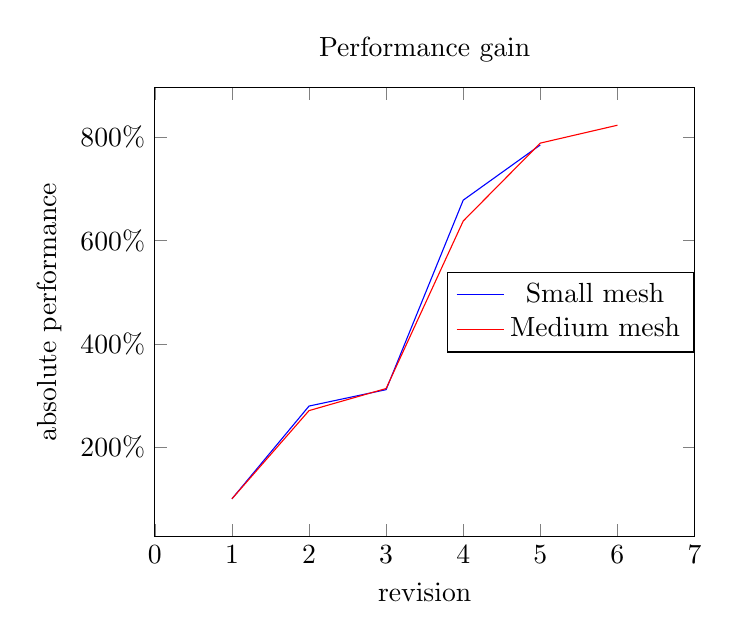
\begin{tikzpicture}
  \begin{axis}[
    legend style={
    at={(1,0.5)},
    anchor=east
    },
    title=Performance gain,
    xmin=0,
    xmax=7,
    enlarge x limits=false,
    ylabel=absolute performance,
    yticklabel={\pgfmathparse{\tick}\pgfmathprintnumber{\pgfmathresult}\%},
    xlabel=revision]
  \addplot[blue] coordinates
    {(1,100.00)  (2,279.58) (3,311.34) (4,678.07) (5,785.00)};
  \addlegendentry{Small mesh}
  \addplot[red] coordinates
    {(1,100.00)  (2,270.77) (3,313.54) (4,637.70) (5,788.53) (6,823.12)};
  \addlegendentry{Medium mesh}
  \end{axis}
\end{tikzpicture}

One of the first hypothesis we rejected almost immediately was to work on cache performance. Cachegrind analysis revealed that the number of cache misses is insignificant and it does not throttle the execution. After performing final evaluation we know that we were right rejecting that theory. We can see that performance increases at the same rate for both small and medium sized mesh. If the application was affected by cache performance we would have noticed it in the performance of the medium sized mesh. No slow down have been observed and we can confirm that cache had little or no effect on the performance.

\vskip 1em
\begin{tikzpicture}
  \begin{axis}[
    title=Comparison of execution time for a small mesh,
    area style,
    ylabel=execution time(s),
    xlabel=measurement,
    enlarge x limits=false]
  \addplot[fill=first] coordinates
    {(0,7.04418)  (1,7.02896) (2,7.00861) (3,6.98379) (4,7.0974)  (5,7.01502) (6,7.06628) (7,6.99485) (8,7.00689) (9,7.16448)}
    \closedcycle;
  \addlegendentry{Rev 1}
   \addplot[fill=second] coordinates
    {(0,2.53058)  (1,2.51935) (2,2.51058) (3,2.51025) (4,2.51287) (5,2.51038) (6,2.52254) (7,2.51972) (8,2.529) (9,2.5193)}
    \closedcycle;
  \addlegendentry{Rev 2}
  \addplot[fill=third] coordinates
    {(0,2.25336)  (1,2.3073)  (2,2.25567) (3,2.24655) (4,2.24741) (5,2.26388) (6,2.24825) (7,2.24406) (8,2.25263) (9,2.29602)}
    \closedcycle;
  \addlegendentry{Rev 3}
  \addplot[fill=fourth] coordinates
    {(0,1.01862)  (1,1.02593) (2,1.02583) (3,1.12799) (4,1.01136) (5,1.02239) (6,1.07915) (7,1.00443) (8,1.03164) (9,1.03658)}
    \closedcycle;
  \addlegendentry{Rev 4}
  \addplot[fill=fifth] coordinates
    {(0,0.902379) (1,0.896919)  (2,0.863794)  (3,0.997336)  (4,0.914804)  (5,0.856639)  (6,0.859562)  (7,0.914349)  (8,0.897033)  (9,0.866656)}
    \closedcycle;
  \addlegendentry{Rev 5}
  \end{axis}
\end{tikzpicture}

\begin{tikzpicture}
  \begin{axis}[
    title=Comparison of execution time for a medium mesh,
    area style,
    ylabel=execution time(s),
    xlabel=measurement,
    enlarge x limits=false]
  \addplot[fill=first] coordinates
    {(0,53.7869) (1, 54.5058) (2,53.9052) (3,54.8274) (4,53.8769) (5,54.7137) (6,53.8338) (7,53.7187) (8,53.7161) (9,53.9564)}
    \closedcycle;
  \addlegendentry{Rev 1}
   \addplot[fill=second] coordinates
    {(0,20.2483) (1, 20.2372) (2,20.1327) (3,19.8411) (4,19.7237) (5,19.7434) (6,20.2217) (7,20.3009) (8,19.7053) (9,19.5902)}
    \closedcycle;
  \addlegendentry{Rev 2}
  \addplot[fill=third] coordinates
    {(0,17.1739) (1, 17.2485) (2,17.2418) (3,17.2849) (4,17.2385) (5,17.2462) (6,17.2613) (7,17.2998) (8,17.2925) (9,17.2096)}
    \closedcycle;
  \addlegendentry{Rev 3}
  \addplot[fill=fourth] coordinates
    {(0,8.3611) (1,8.38078) (2,8.38714) (3,8.24693) (4,8.46204) (5,8.29801) (6,8.30111) (7,8.43508) (8,8.36146) (9,9.5774)}
    \closedcycle;
  \addlegendentry{Rev 4}
  \addplot[fill=fifth] coordinates
    {(0,7.39716) (1, 6.77087) (2,6.77265) (3,6.76595) (4,6.73421) (5,6.89551) (6,6.80409) (7,6.76463) (8,6.82767) (9,6.85561)}
    \closedcycle;
  \addlegendentry{Rev 5}
  \addplot[fill=sixth] coordinates
    {(0,6.58) (1,6.67)  (2,6.56)  (3,6.51)  (4,6.56)  (5,6.51)  (6,6.54) (7,6.72) (8,6.54) (9,6.53)}
    \closedcycle;
  \addlegendentry{Rev 6}
  \end{axis}
\end{tikzpicture}

\begin{sidewaystable}
\centering
Table of execution times used to evaluate performance of the application\\[10pt]
\begin{tabular}{ |c|c|c|c|c|c|c|c|c|c|c|c|c|c| }
  \hline
  Revision & \multicolumn{10}{|c|}{execution time} & average time & absolute performance & relative performance \\
  \hline \hline
  \multicolumn{14}{|c|}{small mesh} \\ \hline
1 & 7.04 &  7.03 &  7.01 &  6.98 &  7.10 &  7.02 &  7.07 &  6.99 &  7.01 &  7.16 &  7.04 &  100.00\% & 100.00\% \\ \hline
2 & 2.53 &  2.52 &  2.51 &  2.51 &  2.51 &  2.51 &  2.52 &  2.52 &  2.53 &  2.52 &  2.52 &  279.58\% & 279.58\% \\ \hline
3 & 2.25 &  2.31 &  2.26 &  2.25 &  2.25 &  2.26 &  2.25 &  2.24 &  2.25 &  2.30 &  2.26 &  311.34\% & 111.36\% \\ \hline
3 & 1.02 &  1.03 &  1.03 &  1.13 &  1.01 &  1.02 &  1.08 &  1.00 &  1.03 &  1.04 &  1.04 &  678.07\% & 217.79\% \\ \hline
5 & 0.90 &  0.90 &  0.86 &  1.00 &  0.91 &  0.86 &  0.86 &  0.91 &  0.90 &  0.87 &  0.90 &  785.00\% & 115.77\% \\ \hline
\hline
\multicolumn{14}{|c|}{medium mesh} \\ \hline
1 & 53.79 & 54.51 & 53.91 & 54.83 & 53.88 & 54.71 & 53.83 & 53.72 & 53.72 & 53.96 & 54.08 & 100.00\% & 100.00\% \\ \hline
2 & 20.25 & 20.24 & 20.13 & 19.84 & 19.72 & 19.74 & 20.22 & 20.30 & 19.71 & 19.59 & 19.97 & 270.77\% & 270.77\% \\ \hline
3 & 17.17 & 17.25 & 17.24 & 17.28 & 17.24 & 17.25 & 17.26 & 17.30 & 17.29 & 17.21 & 17.25 & 313.54\% & 115.80\% \\ \hline
4 & 8.36 &  8.38 &  8.39 &  8.25 &  8.46 &  8.30 &  8.30 &  8.44 &  8.36 &  9.58 &  8.48 & 637.70\% & 203.39\% \\ \hline
5 & 7.40 &  6.77 &  6.77 &  6.77 &  6.73 &  6.90 &  6.80 &  6.76 &  6.83 &  6.86 &  6.86 & 788.53\% & 123.65\% \\ \hline
6 & 6.58 &  6.67 & 6.56 & 6.51 & 6.56 & 6.51 & 6.54 & 6.72 & 6.54 & 6.53 & 6.57 & 823.12\% & 104.39\% \\ \hline
\end{tabular}
\end{sidewaystable}
% trigger a \newpage just before the given reference
% number - used to balance the columns on the last page
% adjust value as needed - may need to be readjusted if
% the document is modified later
%\IEEEtriggeratref{8}
% The "triggered" command can be changed if desired:
%\IEEEtriggercmd{\enlargethispage{-5in}}

% references section

% can use a bibliography generated by BibTeX as a .bbl file
% BibTeX documentation can be easily obtained at:
% http://www.ctan.org/tex-archive/biblio/bibtex/contrib/doc/
% The IEEEtran BibTeX style support page is at:
% http://www.michaelshell.org/tex/ieeetran/bibtex/
%\bibliographystyle{IEEEtran}
% argument is your BibTeX string definitions and bibliography database(s)
%\bibliography{IEEEabrv,../bib/paper}
%
% <OR> manually copy in the resultant .bbl file
% set second argument of \begin to the number of references
% (used to reserve space for the reference number labels box)

% that's all folks
\end{document}